\documentclass[9pt, twocolumn]{article}
\usepackage{graphicx, listings, enumitem, amssymb, url }
\usepackage{color}
\usepackage{multirow, graphicx}

\pagestyle{empty}

\setlength{\textheight}{8.75in}
\setlength{\columnsep}{2.0pc}
\setlength{\textwidth}{6.8in}
%\setlength{\footheight}{0.0in}
\setlength{\topmargin}{0.0in}
\setlength{\headheight}{0.0in}
\setlength{\headsep}{0.0in}
\setlength{\oddsidemargin}{-.19in}
\setlength{\parindent}{1pc}

\definecolor{dkgreen}{rgb}{0,0.6,0}
\definecolor{gray}{rgb}{0.5,0.5,0.5}
\definecolor{mauve}{rgb}{0.58,0,0.82}

\lstset{frame=tb,
  language=Java,
  aboveskip=3mm,
  belowskip=3mm,
  showstringspaces=false,
  columns=flexible,
  basicstyle={\small\ttfamily},
  numbers=none,
  numberstyle=\tiny\color{gray},
  keywordstyle=\color{blue},
  commentstyle=\color{dkgreen},
  stringstyle=\color{mauve},
  breaklines=true,
  breakatwhitespace=true,
  tabsize=3,
  mathescape
}

\makeatletter
\def\@normalsize{\@setsize\normalsize{12pt}\xpt\@xpt
\abovedisplayskip 10pt plus2pt minus5pt\belowdisplayskip \abovedisplayskip
\abovedisplayshortskip \z@ plus3pt\belowdisplayshortskip 6pt plus3pt
minus3pt\let\@listi\@listI} 

\def\subsize{\@setsize\subsize{12pt}\xipt\@xipt}

\def\section{\@startsection {section}{1}{\z@}{24pt plus 2pt minus 2pt}
{12pt plus 2pt minus 2pt}{\large\bf}}

\def\subsection{\@startsection {subsection}{2}{\z@}{12pt plus 2pt minus 2pt}
{12pt plus 2pt minus 2pt}{\subsize\bf}}
\makeatother

\begin{document}

\date{}

\title{\Large\bf Project Report}

\author{
 Ajinkya Rode\hspace{11mm}  Harshit Shah \hspace{11mm}  Ninad Ingale\hspace{11mm} Shikha Soni\\
 ar2443@rit.edu\hspace{5mm} hrs8207@rit.edu\hspace{5mm}  nsi3177@rit.edu\hspace{5mm} srs6573@rit.edu\\
\\
 Computer Science Department\\
 Rochester Institute of Technology\\
 Rochester, NY~~14623
}

\maketitle

\thispagestyle{empty}



\section{Abstract}
{\em
In this paper we present analysis and predictions made using the census income dataset of a country. We have analyzed various hypothesis like the unemployment reasons, region wise industrial development, income tax to the country and few more that are important for making the economical decisions in country. We have used R and Weka for our analysis purpose and PSQL as a database management system. 
%end italics mode
}

\section{Introduction}
Many kinds of datasets are available online but we chose census dataset of a country, considering that there are many things that can be taken under analysis. Various patterns on the basis of their economic information can be predicted. The raw data set that was taken by us had around two hundred thousands entries of the country population including 45 columns like age, sex, education, tax information, and more information on the economic details. 

On careful study of the datasets, we came up with hypotheses such as regionwise industrial and occupational patterns of the country, tax collection, finding out employment status. We came up with these hypotheses in the virtue of understanding various patterns in the population’s economic status. We have built various graphical representations using R, while the classifications have been done in Weka. We have used the J48 algorithm for the classifications. It is a decision tree based algorithm, that produces univariate trees. Also, the J48 classifier displays additional information, including a text representation of the tree it uses to perform evaluations.

\section{Design Considerations}

\subsection{Design Consideration for Database}

\begin{enumerate}
	\item \textbf{ER Diagram:}
		\begin{figure}[ht!]
			\centering
			\includegraphics[width=85mm]{1.jpg}
			\caption{Census Income - ER Diagram}
		\end{figure}
	\item \textbf{Relations, Assumptions, Data Dictionary:}
		\setlist[itemize]{leftmargin=*}
		\begin{itemize}
			\item \textbf{Relations:}
		\par \textit{Person (\underline{p\_id}, age, education, marital\_status, race, hispanic\_origin, sex, labor\_union,
unemployment\_reason, region\_prev\_residence, state\_prev\_residence, household\_family\_stat,
live\_in\_house, citizenship, self\_employed, veteran\_benefits, cob\_father, cob\_mother, cob\_self)} \\
		\par \textit{Employment (\underline{employee\_id}, class\_worker, wage\_phour, industry\_code, occupation\_code, employment\_status, no\_persons\_worked, weeks\_year)}\\
		\par \textit{Person\_Employed (\underline{p\_id}, \underline{employee\_id)}}\\
		\par \textit{Education (\underline{education}, \underline{edu\_high\_qual)}}\\
		\par \textit{Monetary (\underline{m\_id}, capital\_gain, capital\_loss, dividend\_stock, tax\_status)}\\
		\par \textit{Person\_Monetary (\underline{p\_id},m\_id)}\\
		
	\item \textbf{Data Dictionary:}
		\par Here we will briefly discuss the important relations and define the ambiguous column names.\\
%		\setlist[enumerate]{leftmargin=*}
%		\begin{enumerate}
			\par $\rightarrow$ \textbf{Person:}
		\par We have created this relation to store basic personal information like age, education, sex, marital\_status, etc...\\
		\par -$cob\_father$:  Father’s country of birth
		\par -$cob\_mother$: Mother’s country of birth
		\par -$cob\_self$: Person’s own country of birth
		\par -$household\_family\_stat$: Detailed household and family status of a person
		\par -$labor\_union$: If a person is a member of a labor union. (Yes, no or not in universe)
		\par -$live\_in\_house$: If a person lives in the same house 1 year ago
		\par -$region\_prev\_residence$: Region of previous residence of a person (east, west, etc…)
		\par -$state\_prev\_residence$: State of previous residence of a person (east, west, etc…)
		\par -$unemployment\_reason$: Reason for unemployment if person is not working
		\par -$veteran\_benefits$: Person is entitled to veteran’s benefits or not.
		\par -$weeks\_year$: Number of weeks worked in a year\\
		
			\par $\rightarrow$ \textbf{Employment:}
		\par This relation is created to store basic all employment details of a person. This table only contains information about persons who all are employed.\\
		\par -$class\_worker$: Class of a worker like federal government, local government, etc…
		\par -$employment\_status$: Employment status full time, not in labor force, children and armed forces, etc...
		\par -$industry\_code$: Major Industry Code
		\par -$no\_persons\_worked$: Number of persons working for an employer if it is an employer
		\par -$occupation\_code$: Major Occupation Code\\


			\par $\rightarrow$ \textbf{Monetary:}
		\par This relation stores monetary information about an individual. For instance, capital gain/losses and tax filer details.\\
		\par -$capital\_gain$: Capital gains of a person for the specific year
		\par -$capital\_loss$: Capital losses of a person
		\par -$dividend\_stock$: Details about dividends and stocks of a person
		\par -$tax\_status$: tax filer status of a person\\

			\par $\rightarrow$ \textbf{Education:}
		\par Education relation contains person's highest education details and map the highest education with last attended institute. E.g. 9$th$ standard $\rightarrow$ School.\\
\par $edu\_high\_qual$ - Highest education attended like school, college or University
\par $education$ - Highest qualification of a person\\

			\par $\rightarrow$ \textbf{Person\_Employed} and \textbf{Person\_Monetary} relations displays the relationship between \textit{Person} and \textit{Employed}, and \textit{Person} and \textit{Monetary}, tables respectively.\\


%\end{enumerate}

	\item \textbf{Assumptions:}
		\par $\rightarrow$ The attributes, employee\_id and p\_id are foreign keys in Person\_Employed table.
		\par $\rightarrow$ Attributes m\_id and p\_id are foreign keys in Person\_Monetary table.
		\par $\rightarrow$ In the Education table education is a primary key and it is a foreign key in Person table.
		\par $\rightarrow$ One person can be employed for more than one employer.\\
	\end{itemize}

	\item \textbf{Changes made to existing dataset:}
		\par $\rightarrow$ First we have removed columns which contain ambiguous values like $industry\_recode$, $occupation\_recode$. These columns contain numeric values which we were not able to figure out in regards to the industry recodes and they were thus not useful for our analysis.
		\par $\rightarrow$ Another columns $instance\_weight$ and $ignored$  were removed since the former contained numeric values and later had flag values thus making them of no use. So, after removing these columns we were left with 36 attributes.
		\par $\rightarrow$  Furthermore there were columns like $mcc\_msa$, $mcm\_reg$, $msg\_reg$. These columns too had values like `?' making them irrelevant. We removed them along with the other not useful entries. So, we removed these columns and left with 31 columns.
		\par $\rightarrow$ Finally, we have normalized our dataset into six above relations.
\end{enumerate}

\subsection{Design Consideration for Analysis}
%psql, and generated csv
Our data set was of the CSV file format which was easy to load in both R and PSQL. Working on the hypothesis using R was a good option since it is a very good analysis tool which also has amenities to pass SQL queries and make changes in the data. We used the `sqldf' package in R for SQL like querying. But there were certain problems that were faced in using R.\\
\par \noindent $\rightarrow$ \textbf{Problems faced in R for SQL operations}:
\par - Performing DML operations like updating and inserting were difficult
\par - Applying integrity constraints is not possible
\par - Creating a database schema is not possible.\\

To overcome these we decided to use PSQL, for various table related problems, while continue to use R for analytical purposes, and graphical representations. PSQL which is more flexible and has proper data management capabilities was a good option. The whole data was loaded into PSQL after designing the schema and applying the integrity constraints.\\


\par \noindent $\rightarrow$ \textbf{PSQL:}

\par - Inserted the whole data, applying various constraints. 
\par - Removed tuples with the values containing 'Not in universe' Also values like NA were taken care of. Removed these entries since no useful data could be extracted from them. 
\par - The total data dropped down to around 100,000 and this was divided into 6 different tables. 
\par - The tables were studied and normalized into relations.
\par - We added a few columns and made changes o existing columns according to the hypothesis requirements. These will be stated along with each hypothesis .\\


We have used R to analyse the data from different views to identify certain patterns and Weka to obtain specific classification on these extracted $CSVs$.

In a brief we are using PostgreSQL for data extraction and cleaning, R for analysis and Weka for predictive analysis.

%converted into 1 lack records

\section{Analysis and Hypothesis}
\subsection{Employment Status:}
In this analysis we have deduced if a particular person is employed or not based on his/her age, sex, education, citizenship, and marital status information.\\
\par \noindent $\rightarrow$ \textbf{Approach}
\par - Columns used: $education$, $age$, $sex$, $citizenship$, $marital\_status$, $employment\_status$\\
\par - Modifications made to dataset
\par 1) Grouped all $age$ records into four categories, 18, 27, 58 \& 65. Because below the age of 18, the population mainly consists of children, while everybody at the age of 65 or above are the retired ones. Other two groups are 27 and 58. These are made since the number of people with ages around 27 and 58 were in a majority.
\par 2) Grouped $education$ records into three categories. `School Level',`Bachelor's Degree', 'Master's-Doctorate Degree'.
\par 3) Grouped $citizenship$ records into two categories. `US Citizen', `Not a US Citizen'.
\par 4) Grouped $marital_status$ records into two categories. `Married', `Unmarried'.\\
\par \noindent $\rightarrow$ \textbf{Classification}
	\begin{figure}[ht!]
		\centering
		\includegraphics[width=82mm, height=55mm]{h1.jpg}
		\caption{Employment Status}
	\end{figure}

\par \noindent $\rightarrow$ \textbf{Results}

\par It clearly predicted that the population of ages 18 were unemployed since they were children still pursuing education. While the ones above 58 were unemployed possibly since they had retired. \\
\par 1) \textit{Females:}
\par The model strangely predicted that females of the age greater than 27, and are unmarried will be unemployed, while the married US citizens are unemployed. The non US citizens are employed only with a Master’s/doctorate degree, while others are unemployed.
\par Females of ages lesser than 27 and US citizens are employed, while the non US citizens with bachelors degree and Master’s/doctorate degrees are employed while the ones with school degree are unemployed.\\

\par 2) \textit{Males:}
\par Males of age greater than 27 are employed irrespective of their educations. Males with age less than 27 and greater than 18, and if married then all are employed while only unmarried with Master’s/Doctorate degree are employed. So they might still be pursuing their higher education.\\

\par The changes in the person's marital status, citizenship, and education majorly affects the person's employment status.\\



\subsection{Preferred gender in a given industry:}
This hypothesis predicts the preferred gender for any industry on the basis of their age and education. Each industry has their preferences of sex when it comes to the education level, while there are certain industries which prefer either of the sexes, irrespective of the two factors.\\
\par \noindent $\rightarrow$ \textbf{Approach}
\par - Columns used: $education$, $age$, $sex$, $education$, $industry\_code$\\
\par - Modifications made to dataset
\par 1) The education levels and ages are grouped on the same lines as in the above hypothesis. 
\par 2) The industries count was plotted and they were divided into 5 groups on the basis of the descending order of the counts. This graph was plotted in R and shown as below.\\
\par \noindent $\rightarrow$ \textbf{Graph:}
	\begin{figure}[ht!]
		\centering
		\includegraphics[width=85mm]{h2.jpg}
		\caption{Population in the given Industry}
	\end{figure}
\par 3) From the above graph, we grouped all the industries into 5 groups and performed our classification as below. \\
\par \textit{Industries Group 1:}
\par \begin{tabular}{|c| c| }
					\hline
  					Industry & Count\\ \hline
					Manufacturing-durable goods & 9015 \\
					Retail trade & 17070 \\ 
					Education & 8283 \\ 
					Manufacturing-nondurable goods & 6897 \\ \hline
				\end{tabular}\\ \\

\par \textit{Industries Group 2:}
\par \begin{tabular}{|c| c| }
					\hline
  					Industry & Count\\ \hline
					Finance insurance and real estate & 6145 \\
					Construction & 5984 \\ 
					Business and repair services & 5651 \\ 
					Medical except hospital & 4683 \\ 
					Public administration & 4610 \\ \hline
				\end{tabular}\\ \\


\par \textit{Industries Group 3:}
\par \begin{tabular}{|c| c| }
					\hline
  					Industry & Count\\ \hline
					Other professional services & 4482 \\
					Transportation & 4209 \\ 
					Hospital services & 3964 \\ 
					Wholesale trade & 3596 \\ 
					Agriculture & 3023 \\ \hline
				\end{tabular}\\ \\


\par \textit{Industries Group 4:}
\par \begin{tabular}{|c| c| }
					\hline
  					Industry & Count\\ \hline
					Personal services except private HH & 2937 \\
					Social services & 2549 \\ 
					Entertainment & 1651 \\ 
					Communications & 1181 \\ 
					Utilities and sanitary services & 1178 \\ \hline
				\end{tabular}\\ \\

\par \textit{Industries Group 5:}
\par \begin{tabular}{|c| c| }
					\hline
  					Industry & Count\\ \hline
					Private household services & 945 \\
					Mining & 563 \\ 
					Forestry and fisheries & 187 \\ 
					Armed Forces & 36 \\ \hline
				\end{tabular}\\ \\

\par \noindent $\rightarrow$ \textbf{Classification}
	\begin{figure}[ht!]
		\centering
		\includegraphics[width=85mm]{h21.jpg}
		\caption{Industries Group 3}
	\end{figure}\\

\par \noindent $\rightarrow$ \textbf{Results}
\par Looking at the tree in Figure 2, it appears that
\par \textit{Manufacturing non Durable/ Durable goods:} Prefers only Males in industry. 
\par \textit{Retail trade:} Females with school level education and Bachelor level are preferred, provided their ages are less than 18 and greater than 27. Males with ages greater than 18 but less than 27 having school level education, are preferred. Males with the bachelors degree with the age of greater than 27, or with masters degree are preferred. \\
\par \textit{Education:} This industry only prefers the female population.\\
\par The accuracy of our model is 61.9847 \%, which is achieved by training our model on 41265 instances. This accuracy is not up to the mark because  at the very beginning data was cleaned for 'Not in universe' entries and that was a huge amount of data.\\ 


\par In similar way, other four classifications are performed on all other industries groups. Due to space and image quality constraints, we have not included other four decision trees of same hypothesis. From them we can predict the same results as above group, which industries prefer males or females.

\vspace{10mm}

\subsection{Region wise Industrial Development:}
In this hypothesis, region wise industrial development of a country is analyzed based on industry\_code in all four regions. The most influential industry in the country is selected and based upon the occupation\_code for that particular industry\_code, further analysis is done  i.e the majority of population in a particular occupation in a particular region is found.\\

\par \noindent $\rightarrow$ \textbf{Approach}\\
\par - Columns used: $industry\_code$, $curr\_region$, $state\_curr\_residence$, $occupation\_code$\\
\par - Modifications made to dataset:\\
\par 1) A new column, 'state\_curr\_residence' is added with 48 states randomly assigned to employee relation. \\
\par 2) A new column, 'curr\_region' is added containing four regions; North, South, East and West generated on the basis of 'state\_curr\_residence'.\\
\par 3) These added columns, $state\_curr\_residence$ and $curr\_region$ to support our hypothesis and make our analysis more precise.

\par \noindent $\rightarrow$ \textbf{Graph:}
	\begin{figure}[ht!]
		\centering
		\includegraphics[width=85mm]{Western_Region.png}
		\caption{Major industry in a Region}
	\end{figure}\\

\par \noindent $\rightarrow$ \textbf{Graph:}
	\begin{figure}[ht!]
		\centering
		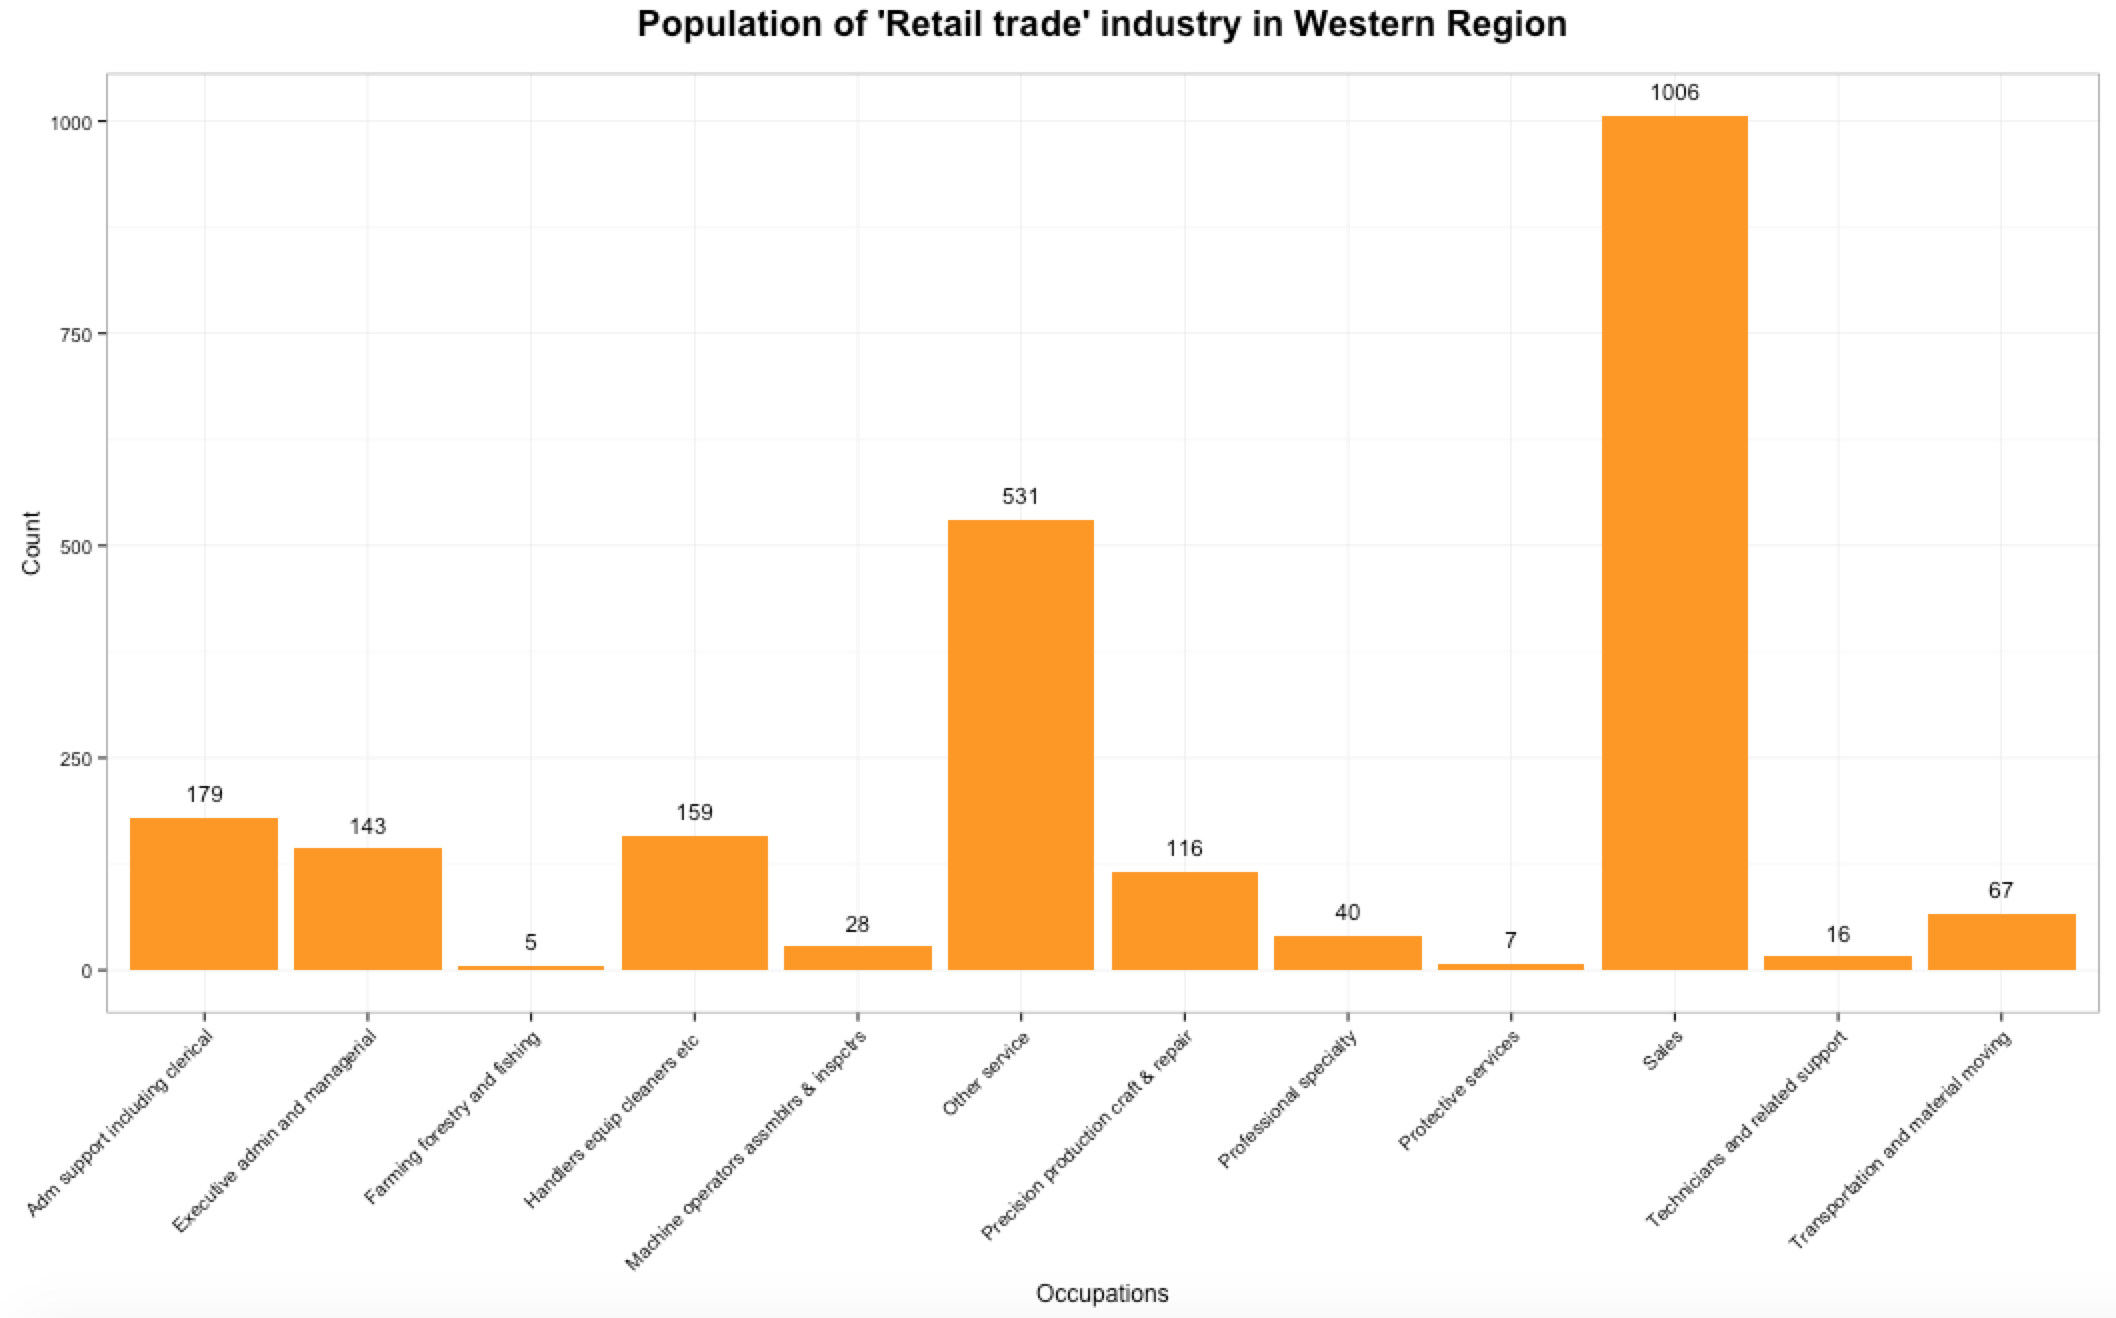
\includegraphics[width=85mm]{Western_Occupation.png}
		\caption{Major occupation in a Region for influential industry}
	\end{figure}
\par \noindent $\rightarrow$ \textbf{Results}
\par 1) From figure 5 we conclude that the major industry in the country in the Western Region is 'Retail Sales'
\par 2) Similarly we generate most influential industry in all four regions. We predict from the figure that 'Retail Sales' is the most influential industry in the whole country.
\par 3) To make this more accurate we drilled down further to find out which all occupations in this industry are mostly preferred
\par 4) From further analysis we found that sales is the major occupation in the Western Reagion. This pattern is followed for all four regions.
\par 5) Hence to conclude, 'Retail Sales' is the major flourishing industry and most of the population chose sales as their occupation in the country.\\

\subsection{Tax Analysis in a country:}
In this analysis we calculate gross income of the country using the wage\_phour and further calculate the income tax of an individual based on his tax\_filer\_status and self generated income-tax rules.\\
\par \noindent $\rightarrow$ \textbf{Approach}
\par - Columns used: $wage\_phour$, $tax\_filer\_status$, $weeks\_year$\\
\par - Modifications made to dataset:
\par 1) A new column, 'annual\_income\_in\_terms\_of\_100k' is added and the annual income of an individual is calculated based on the formula:\\
$annual\_income\_in\_terms\_of\_100k=(wage\_phour*40*weeks\_year)/100000$
\par 2) Here we assume that an individual works for 40 hours per week.
\par 3) The tax that an individual is levied is calculated based on some general tax rules\cite{second}.\\
\par \noindent $\rightarrow$ \textbf{Graph:}
	\begin{figure}[ht!]
		\centering
		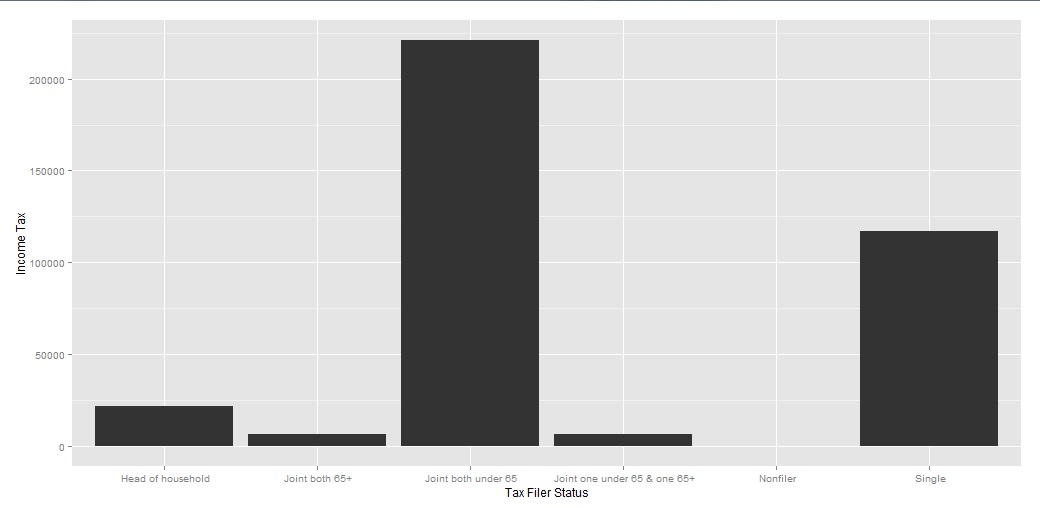
\includegraphics[width=85mm]{Tax_Status.jpg}
		\caption{Income Tax of the Country}
	\end{figure}
\par \noindent $\rightarrow$ \textbf{Results}
\par 1) The most tax paying tax\_filer\_group is 'Joint both under 65'. This is because there is a majority of people from group Joint both under 65 in the dataset at hand.

\subsection{Industry wise Average Annual Income:}
In this analysis we find out the average annual income of a male and female and based on that we find a pattern with respect to industry\_code in the country. \\
\par \noindent $\rightarrow$ \textbf{Approach}
\par - Columns used: $wage\_phour$, $sex$, $weeks\_year$, $industry\_code$\\
\par \noindent $\rightarrow$ \textbf{Graph:}
	\begin{figure}[ht!]
		\centering
		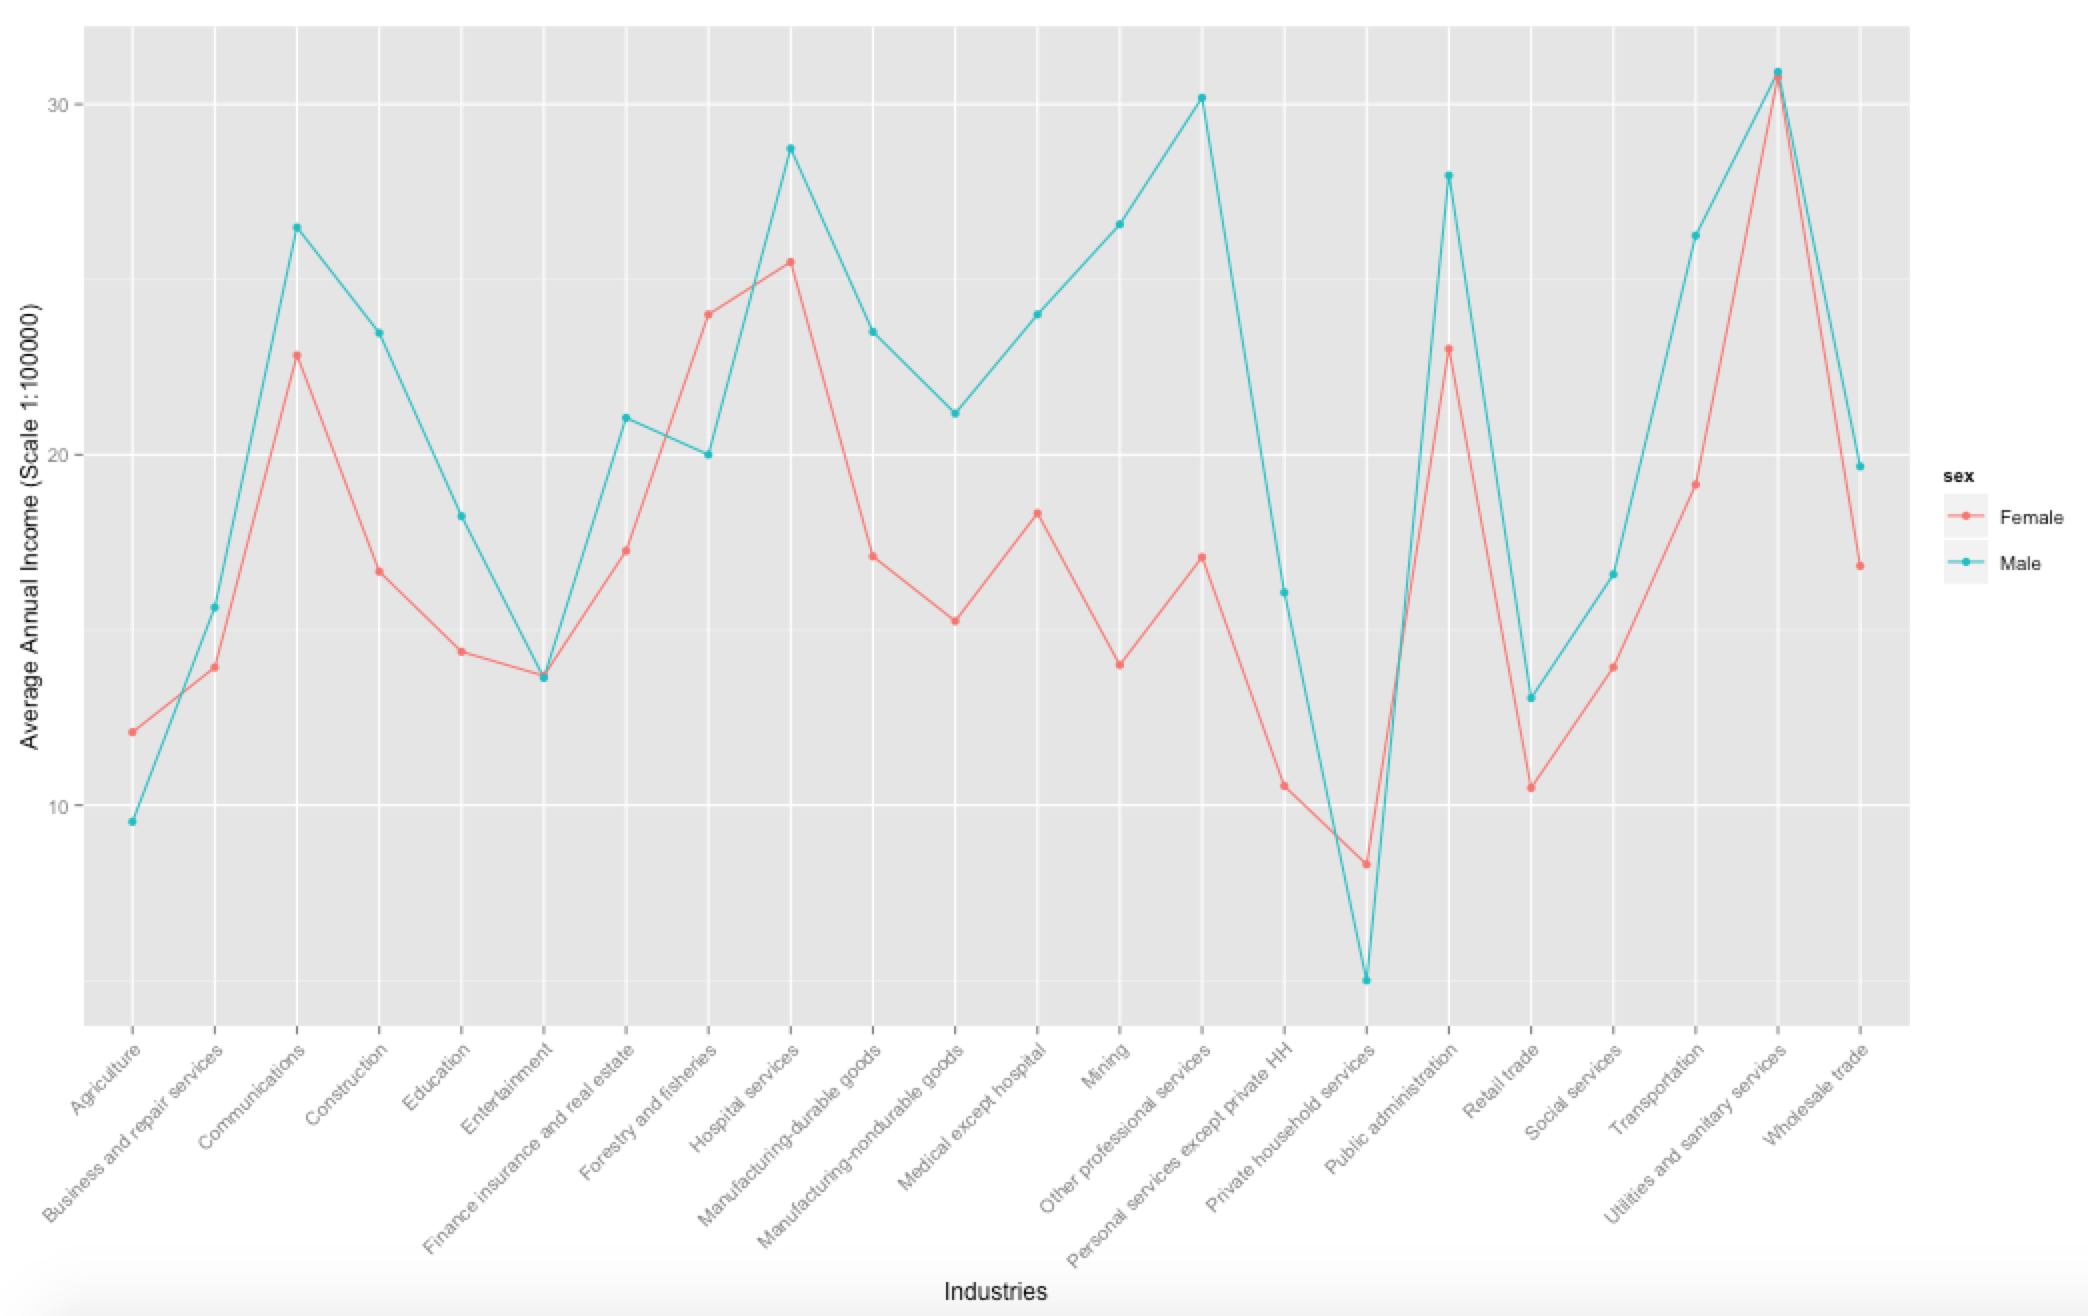
\includegraphics[width=85mm]{Income_Industry.png}
		\caption{Industry wise Average Annual Income}
	\end{figure}

\par \noindent $\rightarrow$ \textbf{Results}
\par 1) Except for fields like Agriculture, Forestry, and Private household services all the industries have males with higher annual income.
\par 2) The industry Utilities and Sanitary services does pay its employees better than other industries.
\par 3) The reasons for females earning higher in these industries are unpredictable.
\par 4) Almost all industries have females with less annual income in each industry by a large margin.


\subsection{Age wise education for particular gender:}
The above graph has been plotted to compare the highest level of education of the population, dividing them sex wise (Male, Female) and age wise(18,27,58,65). Here we are analyzing age wise educated people and comparision between males and females.\\
\par \noindent $\rightarrow$ \textbf{Approach}
\par - Columns used:  $sex$, $education$, $age$ \\
\par - Modifications made to dataset
\par 1) Grouped all $age$ records into four categories, 18, 27, 58 \& 65 as above hypotheses.
\par 2) Grouped $education$ records into seven categories from total availabe sixteen categories for better analysis. Because it is more accurate analysis if we have less categories. The new seven categories are `Pre School-Kindergarten',`Elementary School (1st-4th grade)', 'Middle School (5th-8th grade)', 'High School (9th-12th grade)', 'College or University (Bachelor's Degree)', 'College or University (Master''s-Doctorate Degree)', 'Vocational-Associates Degree'.\\
\par \noindent $\rightarrow$ \textbf{Graph}
	\begin{figure}[ht!]
		\centering
		\includegraphics[width=82mm]{h5.jpg}
		\caption{Age wise education for particular gender}
	\end{figure}

\par In figure 9, the stacked color variations, represents the age group. Where the darkest, at the bottom represents age group of 18, while the lightest, at the top represents age group of 65.\\

\par \noindent $\rightarrow$ \textbf{Results}

\par 1) On studying the graph one obvious thing was covered that the population of ages less than 18 are limited till high school and college university. 
\par 2) On observation the education levels in each group of both the sexes were almost similar.  Majority of the population studied till either high school or completed their bachelor's at the most.
\par 3) People of the age group 58 have studied till their high school or have attained bachelors degree.


\section{Future Work and Lessons Learned}
Working on this project made us familiar with how exactly should a dataset be approached. The various data mining and analysis techniques. We understood how exactly should the bad data be handled, like cleaning the data and getting over the glitches in the important parameters. Exploring tools like R and Weka were extremely helpful. The major challenge we faced was bad data entries. That was overcome and the data was grouped in sets to plot the trees better. \\

In future we can train our model better by improving the accuracy. This can be done if we group the data better, also if we train the model better. Making a user interface for the employment status, unemployment reasons and possible placement of industries on the basis of age and education can be designed to display the project in an interactive way.  

\section{Conclusion}
The project is used to analyze various aspects of the country's economic sector. In conclusion we found out that the employment status of the person, the tax status, region wise industries, preferred sex by a given industry, sex wise annual income. The hypothesis that states the tax information helps find the sector that gives maximum tax thus helping the country predict the tax revenues that could be expected in future. Another important information was where the development of each industry and occupation in the 4 regions could be found, thus helping the nation predict the flourishing states, industries as well as occupations in the country.

\begin{thebibliography}{9}

\bibitem{first}
Lichman, M.  
{\em UCI Machine Learning Repository.} Morgan Kaufmann, (2013).\\
\url{https://archive.ics.uci.edu/ml/datasets/Census-Income+(KDD)}

\bibitem{second}
{\em National Tax Services, Inc.} 2005.\\
\url{http://www.unclefed.com/IRS-Forms/1995-1991/1994TaxRateSchedules.pdf}


\end{thebibliography}

\end{document}
